\section{Аналитическая часть}

\subsection{Представление графической информации в компьютере}

Любая информация, в том числе и графическая, может быть представлена в аналоговой или дискретной форме. При аналоговом представлении физическая величина принимает бесконечное множество значений, причем ее значения изменяются непрерывно. При дискретном представлении физическая величина принимает конечное множество значений, причем ее величина изменяется скачкообразно. Преобразование графической информации из аналоговой формы в дискретную производится путем пространственной дискретизации. Пространственную дискретизацию можно сравнить с построением изображения из мозаики. Изображение разбивается на отдельные маленькие фрагменты (точки), причем каждому фрагменту присваивается значение его цвета, то есть код цвета.

Качество кодирования изображения зависит от двух параметров. Оно тем выше, чем меньше размер точки и соответственно большее количество точек составляет изображение; чем большее количество цветов, то есть большее количество возможных состояний точки изображения, используется.

Графическая информация на экране монитора представляется в виде растрового изображения, которое формируется из определенного количества строк, которые в свою очередь содержат определенное количество точек.

Качество изображения определяется разрешающей способностью монитора, т.е. количеством точек, из которых оно складывается. Чем больше разрешающая способность, т.е. чем больше количество строк растра и точек в строке, тем выше качество изображения. В современных персональных компьютерах обычно используются три основные разрешающие способности экрана: $1920\times1080$, $1336\times768$ и $1536\times864$ точки \cite{screen}.

В простейшем случае (черно-белое изображение без градаций серого цвета) каждая точка экрана может иметь одно из двух состояний -- «черная» или «белая», то есть для хранения ее состояния необходим 1 бит.

Цветные изображения формируются в соответствии с двоичным кодом цвета каждой точки, хранящимся в видеопамяти. Они могут иметь различную глубину цвета, которая задается количеством битов, используемым для кодирования цвета точки. Наиболее распространенными значениями глубины цвета являются 8, 16, 24 или 32 бита. Каждый цвет можно рассматривать как возможное состояние точки, тогда количество цветов, отображаемых на экране монитора, может быть вычислено по формуле:  $N = 2^I$, где I -- глубина цвета.

Цветное изображение на экране монитора формируется за счет смешивания трех базовых цветов: красного, зеленого и синего. Такая цветовая модель называется RGB-моделью.

Для получения богатой палитры цветов базовым цветам могут быть заданы различные интенсивности. Например, при глубине цвета в 24 бита на каждый из цветов возможны $N = 2^8 = 256$ уровней интенсивности, заданные двоичными кодами (от минимальной -- 00000000 до максимальной -- 11111111) \cite{cg}.

\subsection{Выбор грифического формата}

Графический формат определяет способ сохранения графической информации в файле, а также форму хранения информации (используемый алгоритм сжатия). Как и изображения, графические форматы делятся на растровые и векторные. В компьютерной графике применяют, по меньшей мере, три десятка форматов файлов для хранения изображений. Единого формата графических файлов, пригодного для всех приложений, не существует, поэтому имеет место быть проблема сохранения изображений для последующей их обработки. Однако некоторые форматы стали стандартными для целого ряда предметных областей. Крайне важно различать векторные (WMF, DXF, CGM и др.) и растровые (JPEG, PNG, GIF, BMP, ICO и др.) форматы \cite{format}. 

Файлы векторного формата содержат описания рисунков в виде набора простейших графических объектов. В файлах же растровой графики запоминается цвет каждого пикселя на рисунке, поэтому такие файлы занимают, как правило, большой объем памяти. Один из возможных способов решения этой проблемы -- сжатие информации, т. е. уменьшение размеров файла за счет изменения способа организации данных в нем. Обычно каждый конкретный алгоритм хорошо сжимает только изображения вполне определенной структуры.

Для решения задач данной работы был выбран формат BMP.

\subsubsection{Формат BMP}

\textbf{BMP} (полное имя Bitmap) -- это стандартный формат файла изображения в операционной системе Windows, который можно разделить на две категории: зависящее от устройства растровое изображение (DDB) и независимое от устройства растровое изображение (DIB), которое очень широко используется. Он использует формат хранения растровых изображений, в дополнение к дополнительной глубине изображения, не использует никакого другого сжатия, поэтому пространство, занимаемое файлом BMP, очень велико. Глубина изображения файлов BMP может быть выбрана из l, 4, 8, 24 и 32 бит. При хранении данных в файле BMP изображение сканируется в порядке слева направо и снизу вверх. Поскольку формат файла BMP является стандартом для обмена данными, связанными с графиками, в среде Windows, все графические и графические программы, работающие в среде Windows, поддерживают формат изображений BMP \cite{bmp}.

Этот формат был выбран, так как его удобно использовать при создании картинок, которые не теряют качества после их изменений, то есть изображения в этом формате можно редактировать какое угодно количество раз, а их качество ничуть не пострадает (в отличие от того же JPEG).

\subsection{Основные понятия и обработка изображений}

Изображением называется двумерная функция $f(x,y)$ в которой x и у -- координаты в пространстве (на плоскости), а значение функции которой в любой точке, определяется парой координат (х, у), называется интенсивностью изображения в данной точке. Изображение будет являться цифровым, если величины х, у и функция принимают конечное число дискретных значений.

Цифровой обработкой изображений называется обработка цифровых изображений, которые обрабатываются благодаря цифровым вычислительным машинам. Цифровое изображение состоит из конечного числа элементов, каждый из которых расположен в конкретном месте и принимает определенное значение, соответственно называются элементами изображения или пикселями. Для элементов цифрового изображения чаще всего используется термин «пиксель» \cite{imgProc1}. 

Наличие массовой памяти большого объема обязательно для практических задач обработки изображений. Для хранения изображения размером $1024\times1024$ пикселя, в котором яркость каждого пикселя представляется 8-битовой величиной, необходим один мегабайт памяти, если не используются средства сжатия изображений. При работе с тысячами или даже миллионами изображений наличие достаточной внешней памяти в системе обработки изображений может оказаться проблематичным.

Пиксель цифрового изображения является оптически однородным, и внутри его отдельные элементы изображения не выделяются. Экспе-риментально установлено, что для воспроизведения на цифровом снимке компактного объекта его размер должен быть не менее четырех пикселей.

Растровое изображение строится из составляющих его пикселей, размещаемых построчно слева направо и сверху вниз, а доступ к какому-либо из них осуществляется по номеру соответствующего столбца (ix) и строки (jу) \cite{imgProc2}.

Растровые координаты пикселя (ix) и (iy) относятся к его центру, хотя с помощью математического аппарата они могут быть найдены с точностью порядка 0,1 от его размера. В этих случаях для доступа к пикселю используется целая часть его растровых координат.

\subsection{Фильтры обработки изображения}

\subsubsection{Точечные фильтры}

Самый простой фильтр -- это оператор точки. Каждое значение пикселя умножается на скалярное значение. Эта операция может быть записана следующим образом (\ref{fig:dot_for}):
\begin{equation}
	\label{fig:dot_for}
	g(i, j) = K \times f(i, j),
\end{equation}

где:
\begin{itemize}[leftmargin=1.6\parindent]
	\item[---] входное изображение равно F, а значение пикселя в точке (i, j) обозначается как $f(i, j)$;
	\item[---] выходное изображение равно G, а значение пикселя в (i, j) обозначается как $g(i, j)$;
	\item[---] K -- скалярная константа.
\end{itemize}

Этот тип операций с изображением известен как линейный фильтр. В дополнение к умножению на скалярное значение, каждый пиксель также может быть увеличен или уменьшен на постоянное значение \cite{imgProc3}. Таким образом, общая операция с точками может быть записана следующим образом (\ref{fig:lin_for}):

\begin{equation}
	\label{fig:lin_for}
	g(i, j) = K \times f(i, j) + L
\end{equation}

Эта операция может быть применена как к изображениям в оттенках серого, так и к изображениям RGB. Для изображений RGB каждый канал будет изменен с помощью этой операции отдельно. Следующее является результатом изменения как K, так и L. На втором изображении K = 0,5 и L = 0,0, в то время как на третьем изображении K равно 1,0, а L равно 10. Для конечного изображения справа K = 0,7 и L = 25. Как можно заметить, изменение K меняет яркость изображения, а изменение L меняет контрастность изображения (рисунок \ref{fig:spire01}).

\begin{figure}[hbtp]
	\centering
	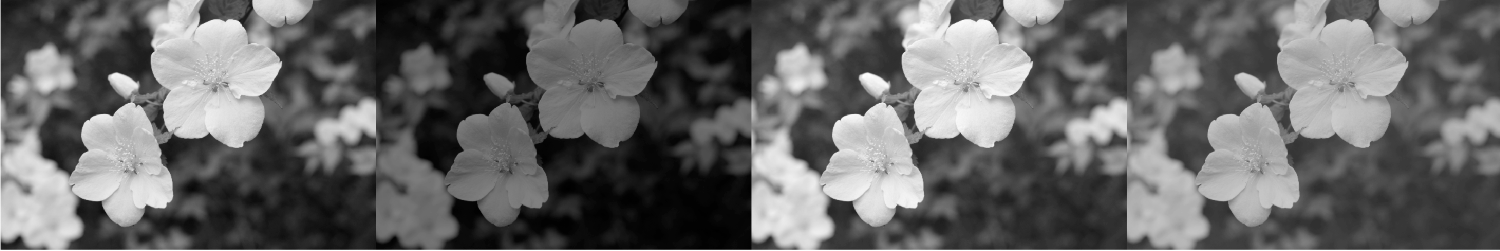
\includegraphics[width=\textwidth]{img/image1.png}
	\caption{\label{fig:spire01} Пример точечной фильтрации}
\end{figure}

\subsubsection{2D линейная фильтрация изображений}

В то время как предыдущий фильтр является точечным фильтром, пиксели изображения также содержат информацию вокруг пикселя. Для извлечения этой информации при фильтрации существует несколько фильтров окрестностей.

Пусть у нас есть следующее исходное изображение (рисунок \ref{fig:spire02}):
\begin{figure}[hbtp]
	\centering
	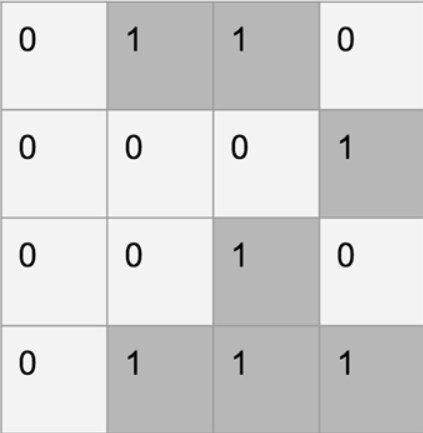
\includegraphics[width=0.5\textwidth]{img/image2.png}
	\caption{\label{fig:spire02} Исходное изображение двойки}
\end{figure}

Это простое двоичное изображение числа 2. Чтобы получить определенную информацию из этого изображения, можно напрямую использовать все значения пикселей. Но вместо этого, для упрощения, можно применить к этому фильтры. Определяется матрицу, меньшую, чем заданное изображение, которая работает в окрестности целевого пикселя. Эта матрица называется ядром, пример такой матрицы представлен на рисунке \ref{fig:spire03}.

\begin{figure}[hbtp]
	\centering
	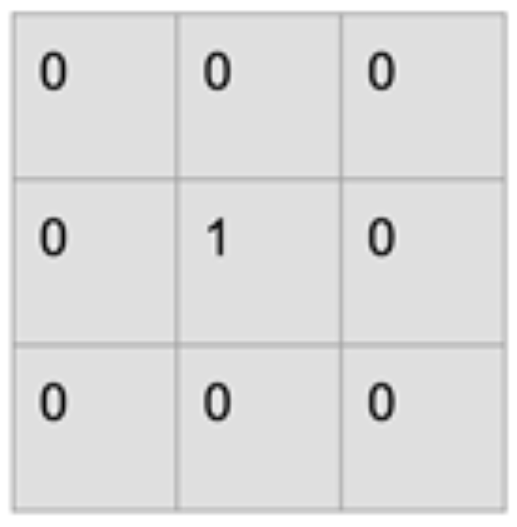
\includegraphics[width=0.3\textwidth]{img/image3.png}
	\caption{\label{fig:spire03} Пример ядра}
\end{figure}

Операция определяется сначала наложением матрицы ядра на исходное изображение, затем взятием произведения соответствующих пикселей и возвратом суммы всех произведений. На рисунке \ref{fig:spire04} нижняя область размером \(3\times3\) в исходном изображении накладывается на заданную матрицу ядра, и соответствующие значения пикселей из ядра и изображения умножаются. Результирующее изображение показано справа и представляет собой суммирование всех предыдущих произведений пикселей:

\begin{figure}[hbtp]
	\centering
	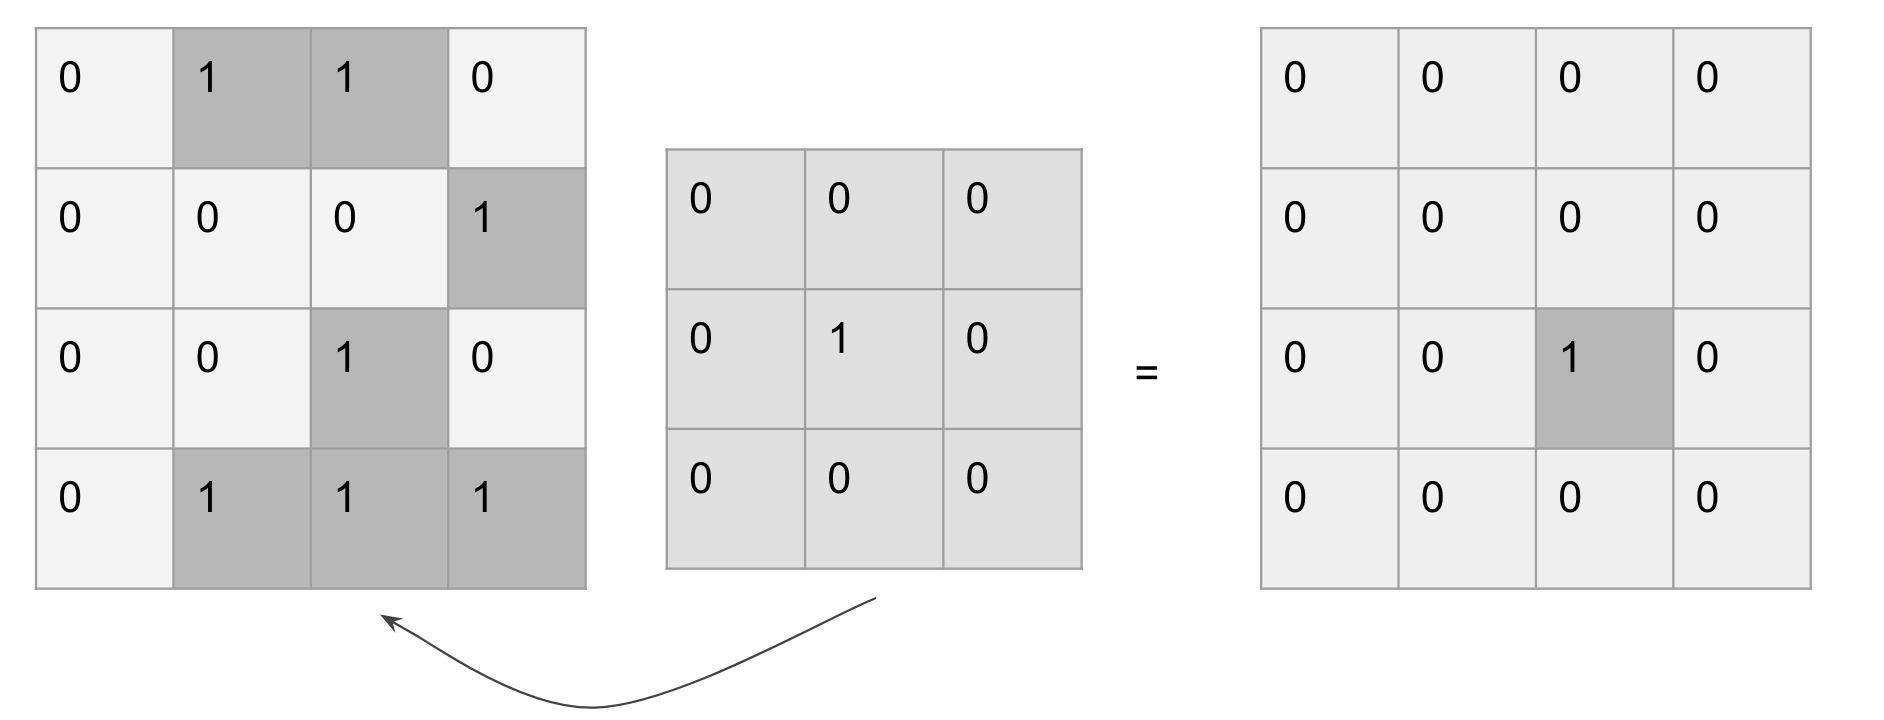
\includegraphics[width=\textwidth]{img/image4.png}
	\caption{\label{fig:spire04} Пример применения матрицы ядра}
\end{figure}

Эта операция повторяется путем перемещения ядра по строкам изображений, а затем по столбцам изображений \cite{imgProc3}. От матрицы свертки зависит результат преобразования изображения.


Ядро фильтра, заданное на прямоугольной окрестности N, может рассматриваться как матрица \(n\times n\), где длины сторон являются нечетными числами. При задании ядра матрицей ее следует центрировать. Если пиксель (x, y) находится в окрестности краев изображения, то координаты A(x-i, y-j) для определенных (i, j) могут соответствовать несуществующим пикселям A за пределами изображения. 

Данную проблему можно разрешить несколькими способами:
\begin{enumerate}[leftmargin=1.6\parindent]
	\item[---] не проводить фильтрацию для таких пикселей, обрезав изображение B по краям, или применив для их значений исходные значения изображения А;
	\item[---] не включать отсутствующий пиксель в суммирование, распределив его вес h(i, j) равномерно среди других пикселей окрестности N(x, y);
	\item[---] доопределить значения пикселей за границами изображения при помощи экстраполяции;
	\item[---] доопределить значения пикселей за границами изображения, при помощи зеркального продолжения изображения.
\end{enumerate} 
Выбор способа производится с учетом конкретного фильтра и особенностей изображения.

\subsubsection{Свойства линейных фильтров}

Несколько приложений компьютерного зрения состоят из пошаговых преобразований входной фотографии в выходной. Это легко сделать благодаря \newline нескольким свойствам, связанным с распространенным типом фильтров, то есть с линейными фильтрами.
\begin{itemize}[leftmargin=1.6\parindent]
	\item[1.] Линейные фильтры являются коммутативными, так что можно выполнять операции умножения над фильтрами в любом порядке, и результат все равно остается тем же:
	\begin{equation}
		a \times b = b \times a.
	\end{equation}
	\item[2.] Они носят ассоциативный характер, что означает, что порядок применения фильтра не влияет на результат:
	\begin{equation}
		(a \times b) \times c = a \times (b \times c).
	\end{equation}
	\item[3.] Даже в случае суммирования двух фильтров можно выполнить первое суммирование, а затем применить фильтр, или также можно индивидуально применить фильтр, а затем суммировать результаты. Общий результат остается прежним.
	\item[4.] Применение коэффициента масштабирования к одному фильтру и умножение на другой фильтр
	эквивалентно первому умножению обоих фильтров, а затем применению коэффициента масштабирования.
\end{itemize}

Эти свойства играют важную роль в других задачах компьютерного зрения, таких как обнаружение объектов и сегментация. Подходящая комбинация этих фильтров повышает качество извлечения информации и, как следствие, повышает точность.

\subsubsection{Нелинейная фильтрация изображений}

Хотя во многих случаях для получения требуемых результатов достаточно линейных фильтров, в нескольких других вариантах использования производительность может быть значительно увеличена с помощью нелинейной фильтрации изображений. Нелинейная фильтрация изображений является более сложной, чем линейная фильтрация. Однако эта сложность может дать вам больше контроля и лучшие результаты в ваших задачах компьютерного зрения. Она позволяет избежать дополнительного искажения изображения при удалении шума, а также значительно улучшить результаты работы фильтров на изображениях с высокой степенью зашумленности \cite{impProc4}.

Основное отличие нелинейного фильтра от линейного заключается в том, что выход нелинейного фильтра формируется нелинейным образом от данных исходного изображения. Линейные фильтры, несмотря на разнообразие производимых ими эффектов, не позволяют проделывать некоторые самые естественные операции. 

Исходные данные нелинейного фильтра и результат фильтрации находятся в логической взаимосвязи, то есть реализуются логическими операциями, такими как максимальный фильтр, минимальный фильтр, средний фильтр и т. д., Путем сравнения значений в определенной окрестности. Для этого нет фиксированного шаблона, поэтому нет конкретной передаточной функции.

Хорошим примером служит пороговая фильтрация. Результатом пороговой фильтрации служит бинарное изображение, определяемое следующим образом (\ref{fig:nonlenear}):

\begin{equation}
	\label{fig:nonlenear}
	g(x, y) = 
	\begin{cases}
		1, &\text{если $f(x, y) > \gamma$}\\
		0, &\text{иначе}
	\end{cases}
\end{equation}

Величина \(\gamma\) является порогом фильтрации. В приложениях используется еще целый ряд простейших нелинейных фильтров. Например, модуль изображения, содержащего пиксели с отрицательным значением, или фильтр, обнуляющий все значения пикселей, меньше данного порога.

\subsection*{Выводы}

Таким образом, можно сделать вывод, что обрабатывать изображения можно различными способами. Все они имеют различную степень сложности и эффективность, поэтому, в программе будут реализованы все тип обработки изображений, описанные выше.

\pagebreak